% ICSE 2027 Technical Track submission.
%
% Format: IEEEtran two-column conference, 10 pt.  Page limit: 10 pages for
% the body + unlimited references (per ICSE Technical Track CFP).
%
% Sibling of 0_main.tex (the manuscript / arXiv version, ACM acmart).
% Both files include the same content fragments (1_introduction.tex, ...),
% but the ICSE version trims for the 10-page two-column budget.
% Use \icsetrim to gate text that should NOT appear in the ICSE submission;
% the macro is a no-op in the arXiv build and \iffalse in this build.

\documentclass[10pt,conference]{IEEEtran}
\IEEEoverridecommandlockouts

\pagestyle{plain}

\usepackage{hyperref}
\hypersetup{
    colorlinks=true,
    linkcolor=blue,
    urlcolor=cyan,
    citecolor=blue,
}
\usepackage{balance}
\usepackage{amsmath,amssymb,amsfonts}
\usepackage{graphicx}
\usepackage{textcomp}
\usepackage{xcolor}
\usepackage{verbatim}
\usepackage{listings}
\usepackage{multirow}
\usepackage{enumitem}
\usepackage{colortbl}
\usepackage{soul}
\usepackage{booktabs}
\usepackage{fancybox}
\usepackage{cite}

% Reuse the color definitions from 0_main.tex.
\definecolor{lightgray}{gray}{0.95}
\definecolor{darkblue}{rgb}{0,0,0.5}
\definecolor{lightred}{rgb}{1, 0.8, 0.8}
\definecolor{lightyellow}{rgb}{1, 1, 0.8}
\definecolor{lightgreen}{rgb}{0.6, 1, 0.6}
\definecolor{mint}{rgb}{0.74, 0.99, 0.79}
\definecolor{forestgreen}{rgb}{0.13, 0.55, 0.13}

% acmart-only macros that may appear in the shared input files; make them
% no-ops in the IEEEtran build.
\providecommand{\Description}[1]{}
\providecommand{\citestyle}[1]{}

% --- Cite vs natbib: 0_main.tex uses \citet via natbib; IEEEtran uses
% standard \cite.  Provide \citet/\citep as aliases so the shared inputs
% compile in both environments.
\providecommand{\citet}[1]{\cite{#1}}
\providecommand{\citep}[1]{\cite{#1}}

% Content gating: \icsetrim{...} drops the argument in this build.  In the
% arXiv build (0_main.tex) we redefine it to be the identity so the
% trimmed content is preserved.
\providecommand{\icsetrim}[1]{}

\begin{document}

\title{License Choice, Prevalence, and Impact in Open Software Projects}

\author{\IEEEauthorblockN{Mahmoud Jahanshahi}
  \IEEEauthorblockA{University of Tennessee\\
    Knoxville, USA\\
    \texttt{mjahan@utk.edu}}
\and
\IEEEauthorblockN{Bogdan Vasilescu}
  \IEEEauthorblockA{Carnegie Mellon University\\
    Pittsburgh, USA\\
    \texttt{vasilescu@cmu.edu}}
\and
\IEEEauthorblockN{Audris Mockus}
  \IEEEauthorblockA{University of Tennessee\\
    Knoxville, USA\\
    \texttt{audris@utk.edu}}
}

\maketitle

\begin{abstract}
The terms of how publicly available source code can be used are dictated
by its license. The license (or its absence), in turn, affects what code
the project may reuse and how its code can be (re)used, and may also
affect external participation and overall activity of the project. We
study license distribution and impact in $131{,}171{,}379$ open-source
projects from World of Code (WoC). We find that $83\%$ lack a formal
license -- four times the rate reported by prior studies that filtered
on stars, maturity, or package-manager presence. Restrictive licenses
have higher retention rates; permissive licenses dominate new adoptions.
We then analyze the $23{,}522$ V2604-aligned projects (about $2.4\%$ of
licensed projects) that underwent a license-type change. Once
pre-treatment popularity (downstream count, upstream count, lifetime
forks) is controlled, the apparent global effects of license direction on
files, blobs, upstream and downstream project counts collapse to
non-significance. The robust finding is language-ecosystem mediation:
C/C++ projects show reduced activity after switching to permissive
licenses, Python projects show the opposite. A year-before/year-after
final-switch reanalysis aligned to WoC V2604 surfaces consistent $\sim
4\%$ attenuations in commits, distinct (bot-filtered) aliased authors,
and sustained activity under restrictive$\rightarrow$permissive
transitions.
\end{abstract}

\begin{IEEEkeywords}
Software license, open source software, license choice, mining software repositories, World of Code.
\end{IEEEkeywords}

\section{Introduction}\label{intro}

Open Source Software (OSS) is a cornerstone of modern software development, providing a collaborative environment that fosters innovation, knowledge exchange, and the widespread use of software tools and libraries. 
The licensing of OSS projects is crucial as it dictates how software can be used, modified, and distributed.
As the number of OSS projects has surged, understanding the intricacies of license selection has become increasingly complex. 

Existing work either lacks the scale or comprehensive identification of licenses to fully reflect license usage in OSS.
More importantly, licence choice, much like the choice of technology~\cite{choice23,ma2020methodology}, may reflect strategic decisions by project maintainers to balance openness, protection, and control over their codebases.
It may also be influenced by matters of technical convenience (e.g., licenses used by the frameworks they depend on), social convenience (e.g., licenses favored by their
collaborators), or simply by awareness, such as the popularity of certain licenses.
% **work backwards from the regresssion predictors to 
% see how they fit within the choice literature and within prior
% license work literature. For example, language and calendar time may be a proxy
% for GPL popularity with older products and C more exposed to  gpl***.

Prior work only tabulated observed license use, but have not attempted to 
% *check* to observe evolution of license type use over time, nor to
model explicitly how the context, such as project size, programming language and other aspects of the project (or individual developer) influence license choice. 

To address these gaps, we aim to develop a model that a) comprehensively accounts for all license types, including minor and non-semantic variations, b) is applied to a sample that approximates the full scale of the OSS ecosystem, and c) incorporates key contextual predictors that may influence differing priorities in license selection among projects and individuals.

The core questions our research seeks to answer are:
\begin{itemize}
    \item \textbf{RQ1}: What are the types, prevalence, and evolution of licenses across the entire open source software landscape?
    \item \textbf{RQ2}: How the characteristics of a project influence the choice of its license?   
\end{itemize}


% While previous research has often emphasized the popularity of
% permissive licenses such as the MIT or Apache licenses, known for
% their flexibility and minimal restrictions, this perspective does
% not fully capture the nuanced landscape of OSS licensing. 
% In particular, the roles of copyleft and weak copyleft licenses,
% which impose stricter conditions to maintain the open nature of
% derivative works, deserve closer examination. 

% To address these complexities, we adopt a data-driven approach,
% analyzing a comprehensive dataset that covers a wide array of OSS
% projects. 
% Our analysis is enhanced by advanced statistical models that account
% for various project characteristics, including the number of
% commits, project maturity, team composition, and file counts. 
% This methodology allows us to identify underlying trends and
% provides a deeper understanding of the factors influencing license
% selection. 


% By addressing these questions, we aim to provide valuable insights
% for developers, project maintainers, and the broader OSS community,
% helping them make informed licensing decisions. 
% These decisions are critical not only for legal compliance and risk
% mitigation but also for sustaining and growing open source
% projects. 

% Our study challenges the prevailing view that permissive licenses are universally favored in OSS by presenting evidence of a more varied licensing landscape.
% We demonstrate that copyleft licenses, often considered restrictive, continue to play a significant role, especially in older and more complex projects.
% Additionally, we emphasize the considerable legal risks posed by the large number of unlicensed projects, highlighting the need for greater awareness and education within the OSS community.

% By illuminating these dynamics, our research contributes to a more profound understanding of the factors that influence license selection in OSS.
% We believe these insights will be pivotal in guiding future research and policy development, ultimately strengthening the legal and operational foundations of the OSS ecosystem.

\section{Theory Development}\label{sec:background}

To theorize about the effects of license choice on a project's performance,
several strands of prior research may be relevant.
First is the line of work on motivations of
individuals~\cite{von2012carrots} and businesses~\cite{Harhoff02} to
participate in OSS.
Second, technical, social, and other factors
that either constraint certain choices in software development or
make them more convenient~\cite{ma2020methodology}.
Third, the specific plans and objectives of the project, and how each license choice may advance and hinder these goals~\cite{sen2008determinants}.

\subsection{Motivations}

\citet{von2012carrots} categorize OSS participant motivations
\icsetrim{into ideology, altruism, kinship, fun, reputation,
reciprocity, learning, own-use, career, and pay}
into ten classes, several of which plausibly influence the type of
licenses contributors prefer (ideology and reciprocity favor strong
copyleft; altruism leans permissive; kinship drives adoption of
licenses already used by collaborators).
\icsetrim{In case of commercial involvement, motivations may diverge
from individual contributors, even if they generally align with profit
maximization~\cite{Harhoff02}. Studies of open and gated software
communities highlight the difficulties firms face in balancing
community-based value creation with private value
appropriation~\cite{Shah06}. However, community sponsorship and
licensing strategies can address these tensions. For instance,
restrictive licenses can ensure long-term control over contributions,
whereas nonmarket\footnote{The term ``nonmarket'' excludes for-profit
organizations.} sponsors might alleviate concerns about the project's
sustainability without the need for restrictive
licenses~\cite{stewart2006impacts}.}
For commercial actors, motivations align with profit maximization
and shape licensing strategy in characteristic
ways~\cite{Harhoff02,Shah06,stewart2006impacts}.
\citet{fershtman2007open} observed empirically that restrictive
licenses attract more contributors per project, while permissive
licenses yield higher productivity per contributor.
\icsetrim{Similarly, research into firm involvement in OSS shows that
licensing choices may be driven by strategic goals. For instance, firms
may adopt permissive licenses to facilitate bundling proprietary and
open source code~\cite{economicos02}. \citet{dahlander2008firms}
identified three strategies firms use to engage with OSS communities:
(1) accessing community development to extend resources, (2) aligning
their strategy with community efforts, and (3) assimilating the
community to integrate and share outcomes. Different commercial models
necessitate distinct licensing strategies. \citet{wagstrom2010impact}
and \citet{zhou2016inflow} identified two types of firm engagement:
community-focused firms (e.g., GNOME), which prioritize building
vibrant OSS communities and monetize through services (which favor
restrictive licenses so that a competitor can not create proprietary
enhancements without sharing the code), and product-focused firms
(e.g., Eclipse), which rely on product revenues and thus favor weaker
copyleft provisions to allow some forms of bundling with proprietary
code.}
Firms differentiate further by engagement model
(\citet{dahlander2008firms}, \citet{wagstrom2010impact},
\citet{zhou2016inflow}): community-focused firms favor restrictive
licenses to prevent third-party proprietary enhancements,
product-focused firms prefer weak copyleft to allow proprietary
bundling.
\icsetrim{Emergence of cloud services endangered the business model of
OSS companies that rely on service contracts. Because cloud companies
provide computing services, they can also run (and sell) the same OSS
software as a service, thus cutting out companies that developed the
software. For example, in 2021, Elasticsearch changed its Apache
license to a commercial one where the products built from that code
can not be provided to others as a managed service. They made another
change in 2024, moving to Affero GPL, which is a copyleft license
that requires anyone running a modified program on a server and
letting other users communicate with it to also provide access to the
source code of the modified version running on the server. As we can
see, the more permissive license (Apache) was changed to a more
restrictive one (commercial, then AGPL), as is typical for the service
model.}

Following \citet{fershtman2007open}'s conjecture:

\begin{itemize}
    \item \textbf{Hypothesis (H1a)}: More restrictive licenses are associated with higher total numbers of authors.
    \item \textbf{Hypothesis (H1b)}: More restrictive licenses (often ideologically motivated) are more likely to be retained.
\end{itemize}

\subsection{Social and Technical Choice}

Licenses, like other technologies and practices, spread through
communities.
Prior studies, such as those by \citet{ma2020methodology} and 
others~\cite{lamba2020heard, choice23}, used the
theory of social contagion~\cite{shoroye2015exploring} to estimate
the impact of exposure, susceptibility, and infectiousness on
developer choices regarding package (and tool) selection.
These studies found
that exposure measured by the number of overall deployments at the
time of choice, had a significant positive effect on 
selection.

By analogy, developers indifferent to or unaware of license
distinctions likely gravitate to licenses they have encountered
(prevalence-driven adoption), and compatibility with collaborators'
existing choices reinforces this (kinship-driven adoption).
\icsetrim{The choice of programming language also influences license
selection due to the culture and practices embedded within specific
developer communities.}
Programming language captures community norms and technical
compatibility: Python and JavaScript projects favor permissive licenses
like MIT or Apache~\cite{lerner2005economics}, while C/C++ projects
tend toward GPL~\cite{fitzgerald2006transformation}.
\icsetrim{The community size associated with a project can also impact
license decisions. \citet{tsay2014influence} found that projects with a
large number of forks are perceived as more valuable and trustworthy by
the community. Projects aiming to encourage collaboration and reuse to
maintain this momentum may favor permissive licenses. Similarly,
\citet{borges2018s} suggest that the number of stars signals community
approval, which, like forks, may influence the choice of more
permissive licenses.}
Community size (forks~\cite{tsay2014influence},
stars~\cite{borges2018s}) and the number of upstream/downstream
projects also plausibly influence license choice, with more interacting
projects favoring balanced (weak-copyleft or conditional) licenses over
extremes. Hence:
\begin{itemize}
    \item \textbf{Hypothesis (H2a)}: License choice is associated with the overall popularity of the license
    at adoption time.
    \item \textbf{Hypothesis (H2b)}: License choice is associated with programming language culture-specific norms.
    \item \textbf{Hypothesis (H2c)}: More permissive licenses are associated with larger community size
    (i.e., more upstream and downstream projects).
\end{itemize}

\subsection{Project Goals}

\icsetrim{While legal compliance sets essential boundaries, the
specific needs and objectives of a project further influence the
selection of an appropriate license. Developers often choose licenses
based on their preferences for the future use of the
software.}
Project-level objectives (e.g., preference for
widespread adoption versus strong copyleft
enforcement~\cite{sen2008determinants}) and the resulting trajectory
\cite{colazo2009impact} also matter.
We use four observable measures to operationalize trajectory:
commit count (activity~\cite{koch2002effort}),
file count (complexity/modularity~\cite{mockus2007large,bird2009putting}),
active-months (maturity~\cite{capiluppi2003characteristics}), and
burstiness (fluctuation, computed as active-months over lifetime).
\icsetrim{Projects with frequent commits tend to have more active
development cycles, making them more reliable and attractive for reuse.
Larger projects with more files are more likely to offer reusable
components, making license choice critical for balancing reuse and
intellectual property protection. Older, more mature projects are
often seen as more reliable, which could be influenced by the choice
of licenses that support long-term sustainability. Projects with high
burstiness may not focus heavily on legal concerns, and instead tend
to choose well-known, widely used licenses.}

\begin{itemize}
\item \textbf{Hypothesis (H3a)}: License choice is associated with project activity, approximated by number of commits.
\item \textbf{Hypothesis (H3b)}: More complex projects (higher number of files and blobs) are more likely to use restrictive licenses.
\item \textbf{Hypothesis (H3c)}: Restrictive licenses are associated with longer-term sustainability, approximated by project activity duration.
\item \textbf{Hypothesis (H3d)}: Burstiness, reflecting fluctuating activity, is associated with more permissive licenses.
\end{itemize}

\section{Comparisons to Prior Work}

Despite legal importance of license choice and the potential to stunt
innovation and poison supply chains, it appears that a significant
portion of OSS participants are ignoring the need to choose a license
or to verify license compatibility. 
We construct a preliminary
theory of how license choice might affect the project by reviewing relevant
literature, operationalizing potential affected factors,
and testing that theory. 
However, while our work is not the first to empirically study software licenses,
it differs from the literature in two important ways.

\textit{Comprehensive Identification of Licenses.}
Most prior research, such as that by \citet{wu2024large} and \citet{xu2023lidetector}, primarily depends on explicit license declarations found in metadata files.
Others, like \citet{feng2019open}, apply static analysis on binaries to detect embedded license texts.
However, these methods may overlook licenses that are not clearly stated or are stored in unconventional directories.
In contrast, we use a comprehensive dataset by \citet{jahanshahi2024license}, 
% which follows a more comprehensive approach 
compiled by scanning virtually the entire OSS ecosystem for any files containing ``license'' in their filepath.
Moreover, the authors use the winnowing algorithm, a robust method for matching license texts to known licenses, enhancing the accuracy of detecting both partial and full matches, even when the text is embedded or slightly modified.
This method captures not only standard license files but also other files potentially holding licensing details, ensuring that no relevant license information is missed.

\textit{Scale and Scope of Analysis.} 
Previous works often limit their scope to specific platforms (e.g., GitHub), a few package manager environments (e.g., NPM), or types of licenses (e.g., OSI-approved licenses), lacking a comprehensive, large-scale approach to detecting and analyzing licenses.
Our study expands this scope by analyzing essentially the entire open source landscape, ensuring a more comprehensive cross-platform understanding of licensing practices.

\icsetrim{In Table~\ref{tbl:litRev}, we compare our study's
methodology, coverage, scope, and scale with the most recent
comparable studies in the field.

\begin{table*}[t]
\centering
\caption{Latest Studies in Open Source Software Licensing}
\label{tbl:litRev}
\resizebox{0.95\textwidth}{!}{
\begin{tabular}{llllr}
    \toprule
    & \textbf{License Detection} & \textbf{Coverage} & \textbf{Scope} & \textbf{Scale} (Projects) \\
    \midrule
    \cite{wu2024large} & Package Manager API & License Files & Maven, NPM, PyPI, RubyGems, Cargo & 3,474,778 \\
    \cite{cui2023empirical} & NLP/Extract License Terms & All Files & GitHub - >1000 Stars & 16,341 \\
    \cite{wolter2023open} & GitHub API+NLP/Extract License Terms & All Files & GitHub - Cataloged by OpenHub & 1,000 \\
    \cite{xu2023lidetector} & NLP/Extract License Terms & All Files & GitHub - Popular Python Projects & 1,846 \\
    \multicolumn{5}{c}{\dotfill} \\
    \textbf{This Study} & \textbf{NLP/Matching Known Licenses} & \textbf{License Files} & \textbf{Entire OSS} & \textbf{131,171,379} \\
    \bottomrule
\end{tabular}}
\end{table*}}
Compared to recent licensing studies
(\citet{wu2024large}: 3.5M projects across 5 package managers;
\citet{cui2023empirical}: 16k high-star GitHub repos;
\citet{wolter2023open}: 1k OpenHub-catalogued repos;
\citet{xu2023lidetector}: 1.8k popular Python repos), our analysis
covers $131$M deforked WoC projects -- two orders of magnitude
larger and not filtered by platform, stars, or package-manager
presence.

\section{Methodology}\label{method}

\subsection{World of Code Infrastructure}

World of Code (WoC)\footnote{https://worldofcode.org} is an infrastructure designed to cross-reference source code change data across the entire FLOSS community, facilitating sampling, measurement, and analysis within and across software ecosystems~\cite{ma2019world,ma2021world}.
In essence, it is a software analysis pipeline that encompasses the discovery and retrieval of data, storage and updates, and the transformations and data augmentation required for downstream analytic tasks~\cite{ma2021world}.

WoC offers various maps that connect git objects and metadata (commits, blobs, authors) to each other.
It also provides higher-level maps, such as project-to-data connections (e.g. project-to-author), author aliasing~\cite{fry2020dataset}, and project deforking maps~\cite{mockus2020complete}. 
We use the project-to-license (P2L) map~\cite{jahanshahi2024license} from WoC that provides all the times at which a license was committed to a project and also verifies whether it still exists in the project latest status\footnote{
Version V, latest at the time of this study.}.
We also employ the concept of deforked projects as introduced by~\cite{mockus2020complete} to avoid potential biases from forks and duplicates of the same project.
Throughout this paper, the term ``project'' refers to this deforked project unless stated otherwise.

\subsection{License Types}

We group licenses based on their characteristics.
This grouping helps categorize and understand the different ways software can be distributed and modified.
These categories typically include permissive, copyleft, weak copyleft, and public domain/unlicensed licenses.
This classification is widely recognized in the field and is supported by various scholarly sources.
As noted by Kaminski and Perry~\cite{kaminski2007open}, these licensing patterns have played a crucial role in shaping the development of OSS.

1. \textit{Permissive Licenses}: These licenses, such as the MIT and BSD licenses, are known for their minimal restrictions on how the software can be used.
These licenses allow software to be freely used, modified, and redistributed, even as part of proprietary software~\cite{kapitsaki2019modeling}.
This permissiveness promotes wider adoption and integration of the software in diverse projects, including commercial applications~\cite{kapitsaki2022help}.

2. \textit{Copyleft Licenses}: These licenses, like the GNU General Public License (GPL), require that any modified versions of the software must also be distributed under the same license.
This ensures that derivative works remain free and open, thus preserving the original freedoms granted by the license~\cite{d2007copyleft}.
This characteristic is essential for maintaining the open source nature of software, as it prevents proprietary modifications~\cite{laurent2012free}.

3. \textit{Weak Copyleft Licenses}: These licenses, such as the GNU Lesser General Public License (LGPL) and Mozilla Public License (MPL), strike a balance between permissive and strong copyleft licenses.
They allow linking with proprietary software under certain conditions, while modifications to the licensed components themselves must remain open~\cite{alamoudi2020open}.
This flexibility encourages the use of open source libraries in both open and closed source projects~\cite{gamalielsson2017licensing}.

4. \textit{Conditional Open Licenses}: These licenses include specific conditions that must be met for usage, such as attribution (CC-BY), non-commercial use, or share-alike requirements.
Creative Commons licenses, like CC-BY and CC-BY-SA, provide a framework for sharing while respecting the creator's conditions~\cite{de2009creative}.

5. \textit{Public Domain/Unlicensed}: Public domain and unlicensed software, including those using the Creative Commons Zero (CC0) license, are not restricted by copyright law.
The authors of such software waive all rights, allowing anyone to use, modify, and distribute the work without any conditions.
This category provides the maximum freedom for software use and is often utilized for simple, non-critical software components.

\subsection{Regression Model}\label{sec:reg}

To address our research question, we selected a regression model appropriate to the nature of our response variable.
Specifically, for RQ2, which investigates whether project characteristics influence their license choice, we use a multinomial logistic regression model.
This model is ideal because the response variable—the license type—is categorical with multiple possible outcomes, allowing us to model the probability of each license type based on project characteristics~\cite{hosmer2013applied}.


\subsubsection{Stratified Sampling}

Since the target population encompasses the entirety of OSS projects and given its scale and heterogeneity, we employed a stratified sampling approach to enhance the representativeness of our sample~\cite{thompson2012sampling}.
We stratified projects using six key variables: the number of commits, the number of blobs, the number of authors, the number of forks, the number of active months, and the earliest commit time of the project.
These variables were selected because they are important indicators of project size, activity, and historical context, which are likely to influence the outcomes of our research~\cite{crowston2005social,koch2002effort}.

\begin{table}[h!]
\centering
\caption{Basic Statistics of Projects in WoC}
\begin{tabular}{l|cccc}
    \toprule
    \textbf{Variable} & \textbf{Minimum} & \textbf{Average} & \textbf{Maximum} & \textbf{Standard Deviation} \\
    \midrule
    NumCommits & 1 & 30.26 & 66,000,003 & 8,611.36 \\
    NumBlobs & 1 & 379.38 & 73,240,796 & 18,053.14 \\
    NumAuthors & 1 & 1.49 & 340,022 & 49.70 \\
    NumForks & 0 & 0.50 & 241,217 & 66.32 \\
    NumActiveMon & 0 & 2.11 & 3,684 & 4.40 \\
    \bottomrule
\end{tabular}
\label{tab:strata}
\end{table}

The WoC's MongoDB project database comprises 131 million OSS projects, and summary statistics for the stratification variables are presented in Table~\ref{tab:strata}.
A notable feature of the data is its heavy right skewness, common in large datasets with many small and inactive projects.
To address this skewness and ensure meaningful strata, we binned each variable as follows:
commits (fewer than 500, 500–2000, and over 2000), blobs (below or above 10,000), authors (one, 2–10, and more than 10), forks (none or at least one), and active months (less than three or more than three). 
These classifications reflect different levels of activity, collaboration, complexity, and community engagement.

Projects were also divided into four historical eras based on their first commit: 
the Foundational Era (before 1998), marking the early stages of open source; 
the Dot-com Boom and OSS Expansion (1998–2010), signifying rapid growth and adoption;
the Maturation and Mainstream Adoption period (2010–2018), when open source became key to enterprise software;
and the Modern Era (2019–present), reflecting recent trends in community engagement and cloud-native technologies.

These stratifications produced 288 unique bins ($3\times 3\times 2\times 2\times 2\times 4$).
We randomly selected 5,000 projects per bin, targeting a total of 1,440,000 projects.
However, due to uneven distribution, some bins contained fewer projects, resulting in a final sample of around 500,000 projects.
Despite this, the large sample size and stratified approach ensure a balanced and comprehensive representation of the OSS ecosystem, supporting robust and generalizable conclusions in our regression analyses.

\subsubsection{Model Variables}

Several project characteristics commonly studied in the literature can affect the choice of license types in open source software (OSS) projects.
Our model includes predictors like the number of commits, blobs, files, stars, authors (core, female, and male), forks, community size, commit times, active months, burstiness, programming language, counts of upstream/downstream projects and blobs, and the delay in adopting a license.
These predictors are based on existing OSS research, indicating their influence on a project's development and decision-making.

\paragraph{Number of Commits} The number of commits is a key indicator of project activity and maintenance.
Koch~\cite{koch2002effort} suggests that projects with frequent commits tend to have more active development cycles, making them more attractive for reuse due to their reliability and continuous improvement.
This ongoing activity may influence license choices to encourage contributions or protect the growing codebase~\cite{koch2002effort}.

\paragraph{Number of Files/Blobs} The number of files or blobs reflects a project's complexity and reuse potential.
Mockus~\cite{mockus2007large} found that larger projects with more files are more likely to provide reusable components, which may influence the choice of a license to balance reuse and protection.
Bird et al.~\cite{bird2009putting} also note that projects with more files, often indicating a modular structure, tend to promote greater community engagement and reuse.

\paragraph{Number of Authors/Core Authors} The number of contributors, including core authors\footnote{
Core authors are those responsible for over 80\% of the project's commits.},
reflects the collaborative nature of an OSS project.
Crowston et al.~\cite{crowston2005social} suggest that projects with more contributors benefit from diverse expertise, leading to higher code quality.
This increased collaboration and quality may influence the choice of a license that promotes fair use and encourages broad community contributions.

\paragraph{Number of Female/Male Authors} Accounting for male and female contributors allows us to explore the role of gender diversity in a project's contributor base.
Gender diversity in OSS projects has garnered attention, with research showing that diverse teams, including gender diversity, often produce higher-quality, more innovative outcomes~\cite{vasilescu2015gender}.
This diversity may influence license choices, particularly those emphasizing inclusivity and community governance.
Projects with more gender-diverse teams might prefer licenses that ensure all contributors feel their work is protected and valued~\cite{terrell2017gender}, shedding light on how social dynamics impact licensing decisions.

\paragraph{Number of Forks/Stars/Community Size} These metrics indicate a project's popularity and community involvement.
Tsay et al.~\cite{tsay2014influence} suggest that projects with more forks are viewed as valuable and trustworthy, which may prompt the choice of a license that fosters collaboration and reuse.
Similarly, Borges et al.~\cite{borges2018s} argue that the number of stars reflects community approval, potentially affecting whether a project adopts a permissive or protective license based on its goals.

\paragraph{Number of Upstream/Downstream Projects/Blobs} An upstream project, from which a project derives code, can heavily influence license choice due to compatibility concerns.
Projects may adopt the same license as their upstream counterparts to ensure smooth integration~\cite{gousios2014exploratory}.
A strong upstream network may also encourage permissive licenses that promote collaboration.
Conversely, downstream projects build on a project's code.
A large number of downstream projects may lead to adopting restrictive licenses, like GPL, to protect the original codebase from misuse~\cite{german2009license}, balancing open use with safeguarding developers' rights.

\paragraph{Earliest/Latest Commit Time, Active Months, Burstiness} These time-based metrics provide insights into a project's maturity and stability.
Capiluppi et al.~\cite{capiluppi2003characteristics} found that older, more established projects with sustained activity are often perceived as stable and reliable, which could influence the selection of a license that supports long-term sustainability goals.

\paragraph{License Adoption Delay} The time lag between a project's initiation and its license adoption can affect the license choice.
Projects that delay adopting a license may do so to better evaluate which license aligns with their evolving goals and community feedback.
This careful consideration helps ensure the selected license supports the project's long-term vision and the needs of its contributors.

\paragraph{Programming Language} The programming language of a project often reflects its technical environment and community culture, influencing licensing preferences.
Languages like Python and JavaScript, popular in web development, tend to favor permissive licenses like MIT or Apache due to their focus on reuse~\cite{lerner2005economics}.
In contrast, languages like C or C++, common in systems programming, may lean toward more restrictive licenses like the GPL, which prioritize keeping derivative works open~\cite{fitzgerald2006transformation}.
Additionally, the choice of language affects compatibility, potentially shaping license decisions to ensure interoperability.

WoC's MongoDB project database tracks file counts by language extension, allowing identification of a project's main language based on the most frequent extension, consistent with standard practices~\cite{vasilescu2015data}.

These factors provide a comprehensive view of OSS projects, covering project characteristics (e.g., number of commits), social dynamics (e.g., author count or gender diversity), and software supply chain relationships (e.g., upstream and downstream projects).
By modeling these predictors, we aim to capture the complexity of OSS licensing decisions and offer insights into how these diverse elements impact license choices.

\section{Results and Discussion}

We organize our results in three parts. 
First, we present a broad exploration of different license types, highlighting 
their prevalence, retention, and general trends.
Next, we detail the regression analysis that examines how the choice of license 
relates to project performance. 
Finally, we focus on the phenomenon of license switching by analyzing performance
metrics before and after a change from permissive to restrictive (or vice versa).

\subsection{The Types and Prevalence of Licenses Across the OSS Landscape}

\subsubsection{Our Findings}

We first counted the total number of projects that had at least one occurrence 
of any license during their lifetime.
We then identified the top 20 most used licenses, 
as shown in Figure~\ref{fig:dis1}.

Out of the 131,171,379 projects indexed by WoC, 22,281,342 projects had at 
least one license committed to their project at some point in their lifetime.
However, when examining the latest version of these projects, 
this number drops to 20,110,256 projects.

When interpreting the numbers shown in these figures, it is important to note 
that the sum of these numbers exceeds the total number of projects with a license.
This discrepancy arises because some projects have multiple licenses and 
are therefore counted in several categories.

\begin{figure*}[t]
\centering
    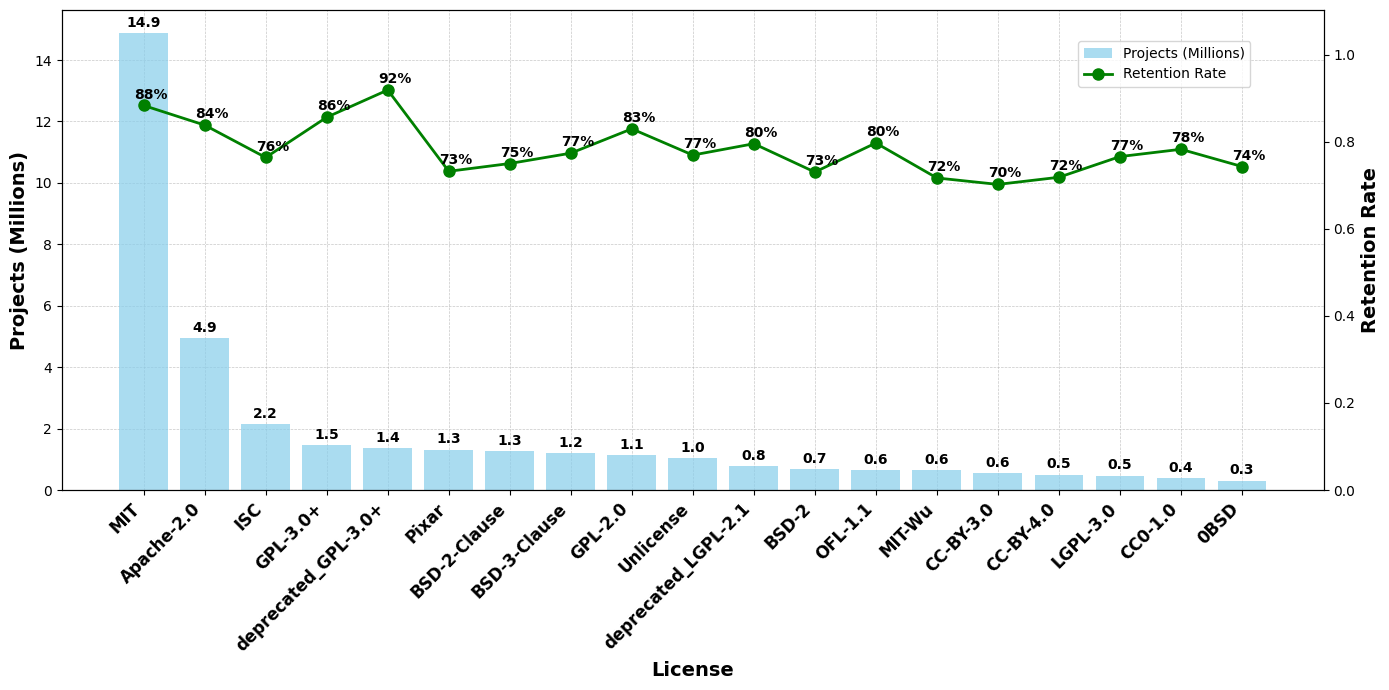
\includegraphics[width=\textwidth]{figures/dis1.png}
    \caption{The distribution and retention rates of the most used licenses.}
    \label{fig:dis1}
    \Description{The distribution and retention rates of the most used licenses.}
\end{figure*}

To calculate the retention rate for each license, we determined the number of 
projects that still had the license in their latest state and divided this number 
by the total number of projects that had ever used the license.
This retention rate indicates the proportion of projects that continue to use 
the license over time, and it is also displayed in Figure~\ref{fig:dis1}.

As shown in the figure, the MIT license is the most prominent, followed
by the Apache 2.0 and ISC licenses.
Notably, per H1b, the deprecated GPL 3 license (with strong
copyleft provisions) exhibits the highest retention rate.
In contrast, the Creative Commons 3 license (CC-BY-3.0) 
shows the lowest retention rate among the top 20 most used licenses.

\begin{figure}[t]
\centering
    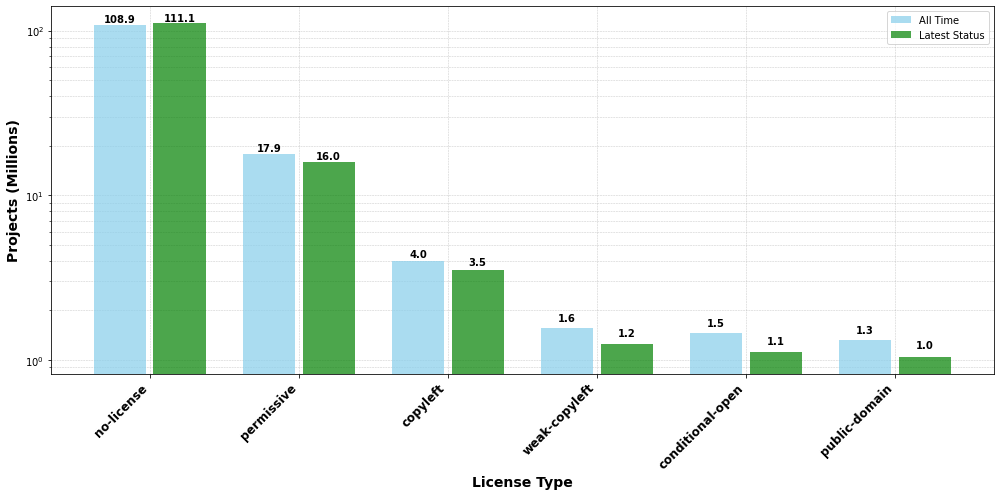
\includegraphics[width=\linewidth]{figures/dis3.png}
    \caption{The distribution of license types across projects.}
    \label{fig:dis3}
    \Description{The distribution of license types across projects.}
\end{figure}

We also analyze the distribution of projects according to their license types.
Initially, we consider the distribution across the entire project history, 
meaning that if a project adopted a license at any point and later removed it, 
it is still counted as having that license.
Next, we determine the distribution based on the most recent status of 
each project.

Figure~\ref{fig:dis3} shows that ``conditional-open'', ``weak-copyleft'', 
and ``public-domain'' license types have the lowest
retention, with approximately a quarter of the projects that ever had 
such license changing it by their latest version.
For comparison, only approximately 8\% of ``copyleft'' licenses were changed, 
which is consistent with our theory (H1b) that ideology-related license choice should be most ``sticky''. 


We also analyze the proportion of adopted licenses at each point in time, 
categorized by license type, to identify trends in licensing preferences over 
time. This allows us to observe shifts in the adoption of different 
licenses and assess whether certain license types have gained or declined 
in popularity. By tracking these proportions longitudinally, we can better 
understand how licensing choices evolve and whether external factors, such 
as regulatory changes or community norms, influence these trends.
Th results are shown in Figure~\ref{fig:proportion}.

\begin{figure}[t]
    \centering
    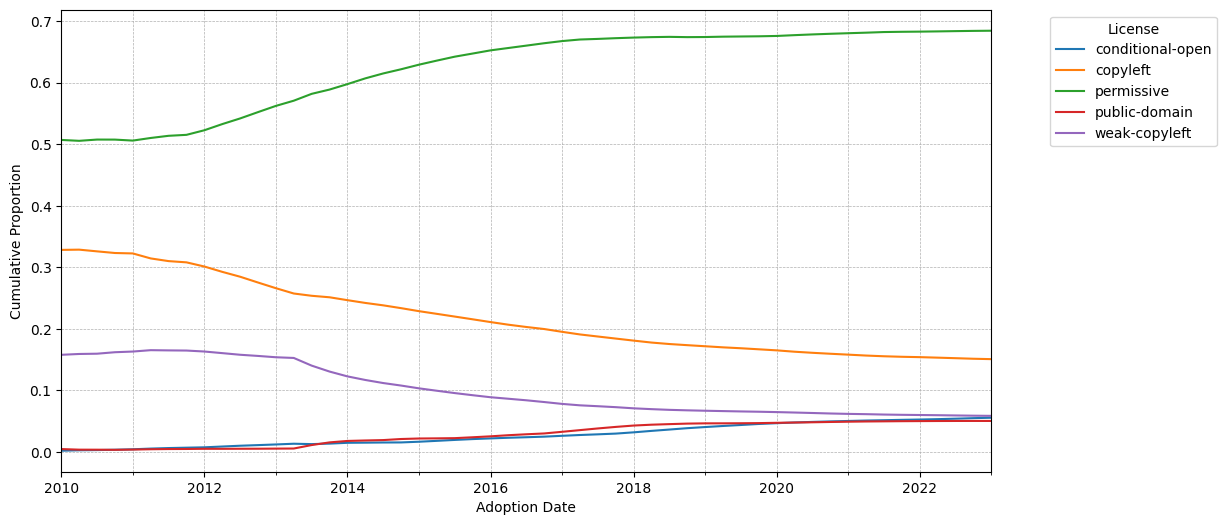
\includegraphics[width=\linewidth]{figures/proportion.png}
    \caption{Proportion of license type over time}
    \label{fig:proportion}
    \Description{Proportion of license type over time}
\end{figure}

Looking at the trends we clearly see that although copyleft licenses
may be the most sticky, the tendency to adopt these licenses has decreased
over time.

\subsubsection{Comparison with Literature}

Table~\ref{tab:res1a} provides a comparison between the results in the 
literature and our study, highlighting substantial differences primarily 
due to variations in scope, methodology, and dataset size 
(see Table~\ref{tbl:litRev}).

\begin{table*}[t]
\centering
\caption{Comparison between our results and the literature.}
\label{tab:res1a}
% \resizebox{0.99\linewidth}{!}{
\begin{tabular}{lrr|rrrrr}
    \toprule
    & \textbf{Projects} & \textbf{No License} & \textbf{Copyleft} & \textbf{Weak} & \textbf{Conditional} & \textbf{Permissive} & \textbf{Public} \\
    & & & & \textbf{Copyleft} & \textbf{Open} & & \textbf{Domain} \\
    \midrule
    \cite{wu2024large} & 3,474,778 & 21.12\% & 5.72\% & 5.12\% & - & 89.16\% & - \\
    \cite{cui2023empirical} & 16,341 & 10.51\% & 11.32\% & 0.97\% & - & 87.71\% & - \\
    \textbf{This Study} & 131,171,379 & 83.01\% & 15.35\% & 5.26\% & 4.82\% & 70.18\% & 4.39\% \\
    \bottomrule
\end{tabular}
\end{table*}


A key methodological difference between our study and \citet{wu2024large} lies in the treatment of data points.
\citet{wu2024large} considered each version of a package as a separate data point, 
resulting in 46.59 million data points from 3.47 million projects.
This approach could introduce bias by overrepresenting projects with many
versions, potentially skewing observed trends in licensing.
Conversely, our study treated each project as a single data point, providing 
a more balanced view of the open source ecosystem without overemphasizing 
projects with frequent updates.

The focus of the \citet{wu2024large} study on only five package managers might explain 
the significant discrepancy in the percentage of projects without a license.
Their study reported that 21.12\% of projects lacked a license,\footnote{
Since the paper provides these percentages by package manager, we calculated the 
overall percentage by taking a weighted average based on the number of 
projects per package manager.} 
whereas our study found a much higher percentage of 83.01\%.
On the other hand, \citet{cui2023empirical} reported that only 10.51\% of
projects were unlicensed.
The difference with \citet{wu2024large} likely stems from the fact that the
package managers they examined are associated with more mature and 
well-maintained projects, which are more likely to have defined licenses.
Additionally, \citet{cui2023empirical} filtered their data to include 
only projects with over 1,000 stars, which might explain why the 
percentage of unlicensed projects is so low\footnote{
These could also be influenced by the differences between OSS projects
and publicly available projects as was explained in the introduction.}.
In contrast, our broader dataset includes a wide variety of projects, many 
of which may be less mature or less formally governed, leading to a higher incidence of unlicensed projects.

The analysis of copyleft versus permissive licenses further reflects 
the differences in scope.
\citet{wu2024large} found a dominance of permissive licenses, with much 
lower percentages for copyleft and weak copyleft licenses.
However, our study, covering all programming languages, reveals a more 
diverse licensing landscape, with a lower percentage of permissive licenses
and higher percentages of copyleft licenses.
This suggests that by focusing on just five package managers, \citet{wu2024large}
might underrepresent broader licensing trends, particularly the prevalence 
of copyleft licenses across the global open source ecosystem.

\begin{figure}[t]
\begin{tcolorbox}[colback=gray!5!white, colframe=gray!70!black, title=Key Findings]
\small
\begin{enumerate}[leftmargin=4mm]
    \item Overall, 83\% of the projects in the dataset lack a formal license, which is significantly higher than the figures reported in previous studies.
    \item The MIT license is the most widely used license,
      accounting for 65\% of all licensed projects and 10\% of all
      OSS projects.
    \item Despite the overall preference for permissive licenses,
      copyleft licenses such as GPL exhibit strong retention rates
      as suggested by H1b.
    \item The differences in license usage reported in our study compared 
    to previous literature highlight the importance of dataset scope 
    and methodology when assessing the prevalence of licenses in OSS projects.
\end{enumerate}
\end{tcolorbox}
\Description{Key Findings}
\end{figure}

\subsubsection{Implications}

The analysis of public repository licensing reveals that 83\% of projects lack a
formal license, posing significant legal risks and discouraging
innovation by preventing responsible actors from reusing unlicensed code. 
This highlights the need for developers to prioritize licensing to set 
clear terms of use.
Our findings challenge previous studies, which often underestimate the 
prevalence of unlicensed projects by focusing on mature ones, missing 
the broader risks of software reuse.

Even though many of these unlicensed projects may seem trivial and 
technically not OSS, their 
public availability still creates legal ambiguity and poses a risk 
of license noncompliance, especially when combined with the lack of 
thorough legal review in many downstream projects.
\citet{jahanshahi2024beyond} demonstrated that in the context of 
copy-based reuse, nearly 18\% of reused artifacts originated from 
very small projects,\footnote{
Projects with no stars and fewer than 10 commits.
} while large projects\footnote{
Projects with more than 10 stars and 100 commits.
} accounted for only 32\% of reused artifacts.
This highlights the importance of addressing the issue of unlicensed code within the OSS ecosystem.

Among projects that are licensed, the MIT license is the most prevalent, 
reflecting a historic preference for permissive licenses that facilitate 
broad adoption and collaboration.
However, the continued use of copyleft licenses like the GPL
(which was popular decades ago)
demonstrates that many developers are committed to preserving the
open nature of derivative works.

\subsection{The Impact of License Choice on Project Characteristics}

\subsubsection{Our Findings}

Now we turn to the results of our regression model discussed in Section~\ref{sec:reg}.
The basic statistics of the response and control variables, including the 
5th percentile, median, mean, and 95th percentile for the numeric variables, 
as well as the counts of different levels for the factor variables, 
are presented in Table~\ref{tbl:stat-l}.

\begin{table*}[t]
\centering
\caption{License type model - descriptive statistics.}
\resizebox{0.99\textwidth}{!}{
\begin{tabular}{cllcccc}
  \toprule
  & \textbf{Variable} & \textbf{Description} & & \textbf{Statistics} & & \\ 
  \midrule
  \midrule
  \multirow{9}{*}{\rotatebox{90}{\textbf{Response}}} 
  & & & \textbf{5\%} & \textbf{Median} & \textbf{Mean} & \textbf{95\%} \\ 
  & LatestCommit & Time since the latest commit & 04/30/2011 & 02/17/2020 & 03/15/2019 & 04/28/2023 \\
  & Active Month & Number of active months & 1 & 7 & 21.65 & 88 \\
  & Burstiness & (Latest - Earliest) / Active months & 0 & 1 & 1.87 & 6.37 \\
  & Authors & Number of authors & 1 & 2 & 23.31 & 56 \\
  & Commits & Number of commits & 2 & 155 & 2,982.63 & 5,770 \\
  & UpProjects & Number of upstream projects & 1 & 44 & 209.21 & 875 \\
  & DownProjects & Number of downstream projects & 0 & 12 & 1,831.07 & 2,342 \\ 
  & Files & Number of files & 5 & 1,820 & 17,295.57 & 59,939.60 \\ 
  & Blobs & Number of blobs & 15 & 5,616 & 19,952.34 & 51,076 \\
  \midrule
  \multirow{5}{*}{\rotatebox{90}{\textbf{Control}}} 
  & EarliestCommit & Time since the earliest commit & 05/08/2006 & 07/05/2017 & 01/31/2016 & 11/23/2021 \\
  & AdoptDelay & Earliest commit to license adoption (days) & 0 & 0 & 133 & 751 \\ 
  \multicolumn{6}{c}{\dotfill} \\
  & Language & \hspace{-0.2cm}JavaScript \hspace{1.15cm} C/C++ \hspace{1.1cm} Python & Java & PHP & Ruby & (Remaining) \\ 
  & Counts (\%) & \hspace{-0.6cm}221,588 (38.72\%) \hspace{0.1cm} 82,551 (14.43\%) \hspace{0.1cm} 53,468 (9.34\%) & 50,372 (8.80\%) & 44,952 (7.86\%) & 18,592 (3.25\%) & 100,650 (17.59\%) \\ 
  \midrule
  & License & \hspace{0.0cm}No License \hspace{1.5cm} Permissive & \hspace{-1.3cm} Copyleft & Weak Copyleft & Conditional Open & Public Domain \\ 
  & Counts (\%) & \hspace{-0.35cm} 263,974 (46.13\%) \hspace{0.7cm} 148,320 (25.92\%) & \hspace{-1.2cm} 60,925 (10.65\%) & 43,143 (7.54\%) & 30,933 (5.41\%) & 24,878 (4.35\%) \\
  \bottomrule
\end{tabular}}
\label{tbl:stat-l}
\end{table*}

Given that we have multiple response variables, the model provides a distinct set of coefficients for each outcome.
Each set of coefficients indicates the influence of the predictor variables 
on the probability of the response variable assuming that there might 
be correlation between response variables.

For categorical variables, we employed sum contrasts, also known as effect 
coding, where each level of the predictor variable is compared to the 
overall mean of all levels.
This approach is particularly advantageous in models where the goal is to 
compare each category to the overall mean rather than to a specific 
reference category, as it offers a more symmetric interpretation of the effects.
In the sum contrast method, the sum of the coefficients for all levels, including the intercept, must equal zero.
We also include the interaction term between language and license in the model.

Furthermore, in interpreting the earliest and latest commit times, it is important to emphasize that the predictors used in the model represent the time elapsed since those commits.
This means that a higher value for the earliest commit indicates that the commit occurred further in the past (i.e., the project is older), and a lower value indicates a more recent commit.

Table~\ref{tbl:anova-l}) shows Type III MANOVA Tests with Pillai test statistic
for the fitted model. 
The results show that the p-values for all the predictors are close to zero, 
indicating that each predictor significantly improves our model's fit.

\begin{table}[t]
\centering
\caption{License choice model - Type III MANOVA Tests: Pillai test statistic}
% \resizebox{\linewidth}{!}{
\begin{tabular}{lccc}
    \toprule
    \textbf{Variable} & \textbf{DF} & \textbf{Test Stat} & \textbf{p.value} \\ 
    \midrule
    (Intercept) & 1 & 0.29263 & \cellcolor{lightgreen}$<2\times10^{-16}$ \\
    License & 5 & 0.04443 & \cellcolor{lightgreen}$<2\times10^{-16}$ \\
    Language & 11 & 0.09268 & \cellcolor{lightgreen}$<2\times10^{-16}$ \\
    EarliestCommit & 1 & 0.60320 & \cellcolor{lightgreen}$<2\times10^{-16}$ \\
    Delay & 1 & 0.11327 & \cellcolor{lightgreen}$<2\times10^{-16}$ \\
    License:Language & 55 & 0.07032 & \cellcolor{lightgreen}$<2\times10^{-16}$ \\
    \bottomrule
\end{tabular}
\label{tbl:anova-l}
\end{table}


\begin{figure*}[t]
    \centering
    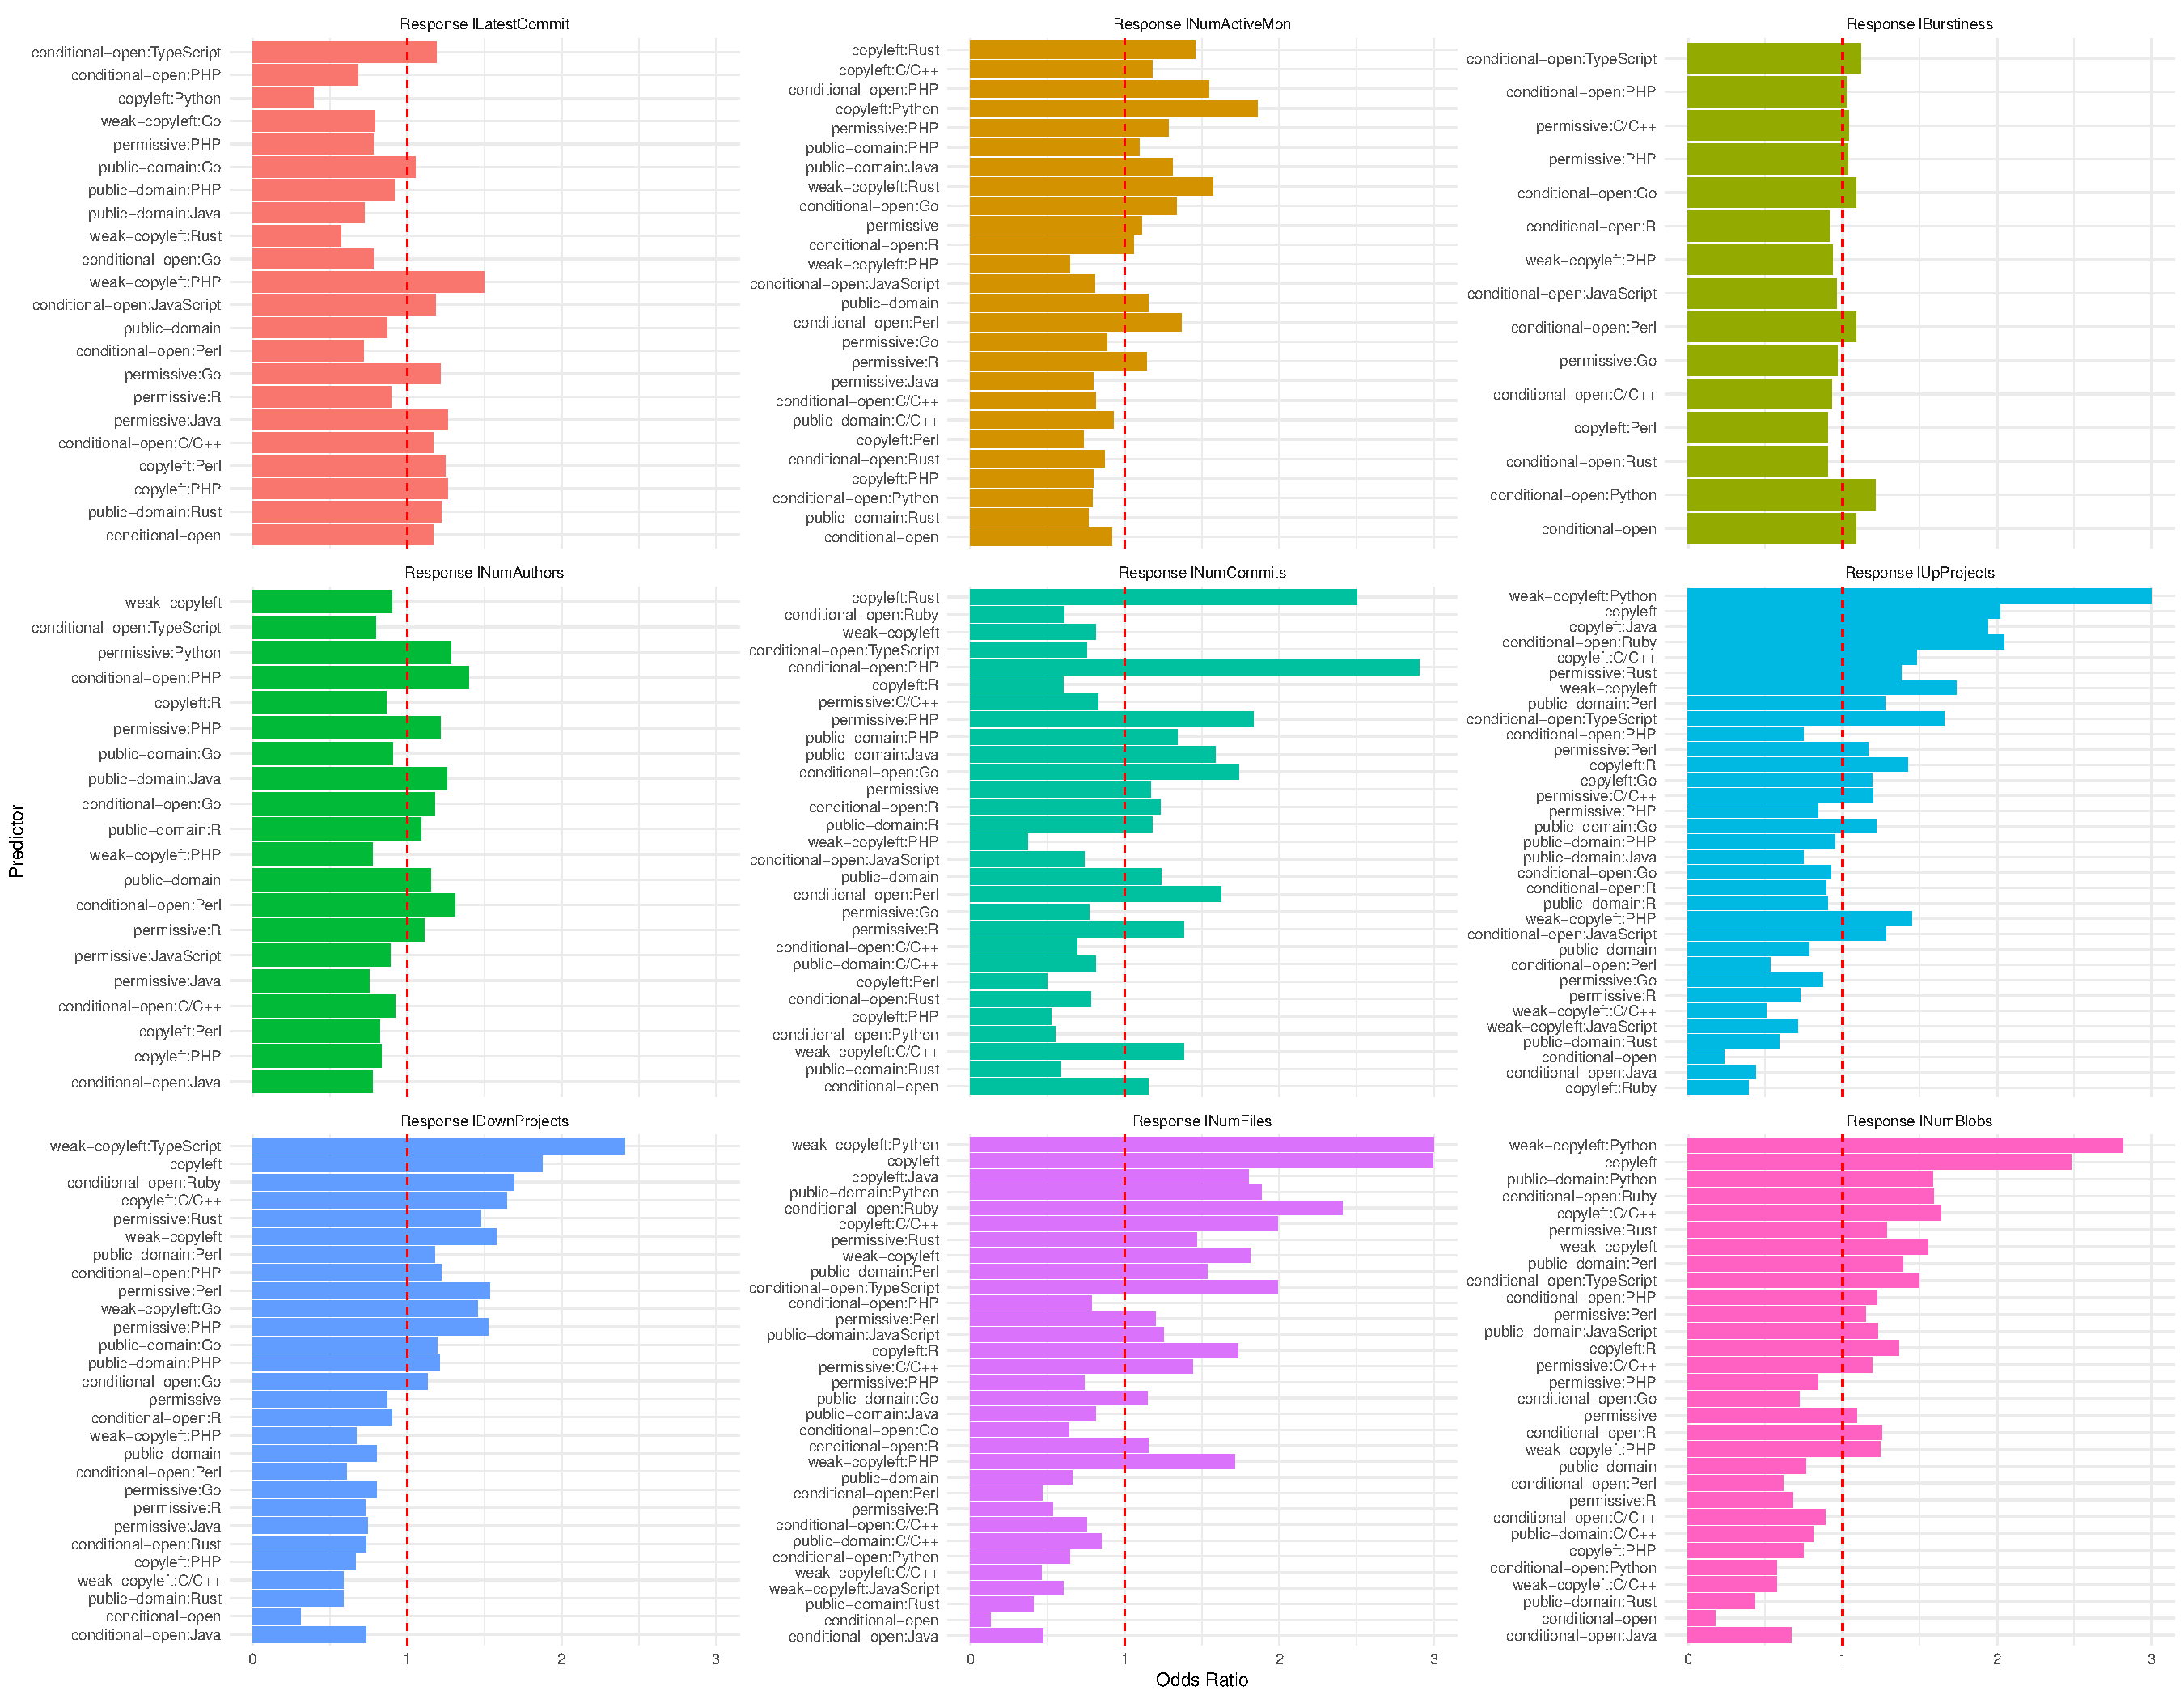
\includegraphics[width=\linewidth]{figures/odds_ratio_plot.pdf}
    \caption{License choice model - odds ratios}
    \label{fig:probs}
    \Description{License model - odds ratios}
\end{figure*}


%%%%%%%%%%%%%%%%%%%%% H1 %%%%%%%%%%%%%%%%%%%%%



%%%%%%%%%%%%%%%%%%%%% H2 %%%%%%%%%%%%%%%%%%%%%

Our analysis shows significant variation in licensing preferences
across programming languages, reflecting the community culture and
technical norms associated with each language (as predicted by H2a).
JavaScript, Ruby, TypeScript, and Go exhibit a strong preference for
permissive licenses (e.g., MIT, Apache), likely due to their
dominant role in web development and collaborative environments or
because these communities started from using such licenses. 
Conversely, Perl, R, and C/C++ favor copyleft licenses (e.g., GPL),
aligning with their historical ties to the early days of open-source movement when
copy-left licenses were more common (H2a) (see Figure~\ref{fig:proportion}).

As the number of forks increases, projects show a clear shift toward
permissive licenses, with the likelihood rising from 55.26\% to
60.10\%, while the adoption of copyleft and conditional licenses
declines slightly. 
This supports the H2b that projects with more forks, perceived as valuable by the community, tend to prioritize collaboration and reuse by favoring permissive licenses.

For downstream projects, the likelihood of selecting conditional open,
public domain, and weak copyleft licenses increases modestly. 
Meanwhile, both permissive and strong copyleft licenses see a 
slight decline. This suggests that developers with more downstream 
interactions are leaning toward less restrictive licenses, supporting H2b.
This is 
reflected by the decrease in strong copyleft and increase in weak 
copyleft, possibly driven by motivations similar to Hypothesis H1c. 
Additionally, the increase in public domain licensing and decline 
in permissive licenses may also reflect a shift toward even 
fewer restrictions.

%%%%%%%%%%%%%%%%%%%%% H3 %%%%%%%%%%%%%%%%%%%%%

% delay
As the delay in adopting a license increases (from 1 to 12 months),
projects show a slight increase in the likelihood of selecting
conditional open, public domain, and weak copyleft licenses. 
Meanwhile, the probability of choosing a permissive license
decreases.
This suggests that longer delays allow more time for legal and
community considerations, leaning towards less known licenses.
The probability of selecting a copyleft license remains stable,
suggesting it is less influenced by the timing of the decision. 
Overall, our hypothesis H3a that more delay translates in less common
license is confirmed, as the permissive and copyleft licenses are
the most used (known) licenses in OSS. 

%%%%%%%%%%%%%%%%%%%%% H4 %%%%%%%%%%%%%%%%%%%%%

As project activity increases, reflected by the number of commits, there is a rise in the adoption of copyleft and permissive licenses, with the probability of conditional open and public domain licenses decreasing.
This suggests that projects with more frequent development cycles
may lean toward either protection via copyleft or flexibility via
permissive licenses. While this partially supports H4a, that too permissive 
licenses (e.g. public domain) will not be favored, the increase in strong copyleft
contradicts our hypothesis.

For larger projects, as measured by the number of files, there is a 
notable increase in weak copyleft licenses, while permissive licenses 
see a sharp decrease. This suggests that as complexity grows, 
developers may prefer licenses that offer more control and protection, 
aligning with the hypothesis that larger, modular projects balance 
reuse with intellectual property concerns, supporting H4b. 
In contrast, conditional open, public domain, and strong copyleft 
licenses show only modest increases.

Older projects, as indicated by the time since the earliest commit,
show a preference for copyleft licenses, while newer projects are
more likely to adopt permissive or conditional open licenses (H4c). 
This reflects the hypothesis that mature projects may seek
sustainability and protection, while newer projects prioritize rapid
contributions or, that older projects, at theirs start, were relatively more
exposed to copyleft licenses (H2a, see Figure~\ref{fig:proportion}).



Inactive projects, marked by longer time since the latest commit,
show slight increases in conditional open, copyleft, and weak
copyleft licenses, while permissive and public domain licenses
decrease. 
This suggests that flexible licenses may correlate with continued
activity, while more restrictive licenses become prevalent as
projects age. This could also be the result of older projects
leaning toward more restrictive licenses.

In bursty projects (those with fluctuating activity), both
permissive and copyleft licenses increase slightly, reflecting the
dual need for flexibility and protection.
This aligns with the hypothesis that bursty projects may prefer
licenses that are more popular and used in many other projects (H4d).

\begin{comment}
As theorised, software project licensing preferences are influenced by
various factors, including the number of commits, files, core
authors, female authors, forks, downstream projects, project age,
and activity levels.

As commits increase, projects tend to favor copyleft and permissive licenses, while conditional open, public domain, and weak copyleft licenses become less common.
In contrast, projects with more files shift away from permissive licenses toward conditional open, public domain, and weak copyleft licenses, with copyleft licenses remaining stable.

The number of core authors slightly reduces the likelihood of adopting conditional open, copyleft, and public domain licenses, while permissive licenses gain a slight preference.
Projects with more female authors tend to adopt conditional open and public domain licenses more frequently, with a corresponding decline in copyleft and permissive licenses.

As forks increase, there is a clear preference for permissive licenses, while conditional open, copyleft, public domain, and weak copyleft licenses decrease.
Similarly, as downstream projects grow, developers lean toward licenses with more specific conditions for control and protection.

Over time, older and inactive projects shift from permissive and conditional licenses to copyleft and weak copyleft, while projects in bursty development environments slightly favor permissive licenses for their simplicity.

Ultimately, licensing choices are shaped by cultural, historical, and practical factors.
Permissive licenses dominate many programming languages due to their flexibility, while copyleft licenses are preferred in communities that prioritize long-term software freedom.
Language-specific use cases and historical context also play a key role in shaping these preferences.
\end{comment}

\subsubsection{Comparison with Literature}

Table~\ref{tab:res1b} provides a comparison between the results in the literature and our study, highlighting substantial differences primarily due to variations in scope and sampling strategy.

\begin{table*}[t]
\centering
\caption{Comparison with literature}
\label{tab:res1b}
\resizebox{0.99\textwidth}{!}{
\begin{tabular}{lllr|rrrrr}
    \toprule
    \multirow{2}{*}{\textbf{Language}} & \multirow{2}{*}{\textbf{Study}} & \multirow{2}{*}{\textbf{Mode}} & \multirow{2}{*}{\textbf{Projects}} & \multirow{2}{*}{\textbf{Copyleft}} & \textbf{Weak} & \textbf{Conditional} & \multirow{2}{*}{\textbf{Permissive}} & \textbf{Public} \\
    & & & & & \textbf{Copyleft} & \textbf{Open} & & \textbf{Domain} \\
    \midrule
    \multirow{3}{*}{\textbf{Java}} & \cite{wu2024large} & Observed & 513,939 & 5.00\% & 21.25\% & - & 73.75\% & - \\
    & \multirow{2}{*}{\textbf{This Study}} & Observed & \multirow{2}{*}{50,372} & 22.25\% & 18.01\% & 1.84\% & 56.79\% & 1.11\% \\
    & & Model & & 20.59\% & 13.53\% & 1.33\% & 63.66\% & 0.84\% \\
    \multicolumn{8}{c}{\dotfill} \\
    
    \multirow{3}{*}{\textbf{JavaScript}} & \cite{wu2024large} & Observed & 2,182,959 & 3.75\% & 1.88\% & - & 94.38\% & - \\
    & \multirow{2}{*}{\textbf{This Study}} & Observed & \multirow{2}{*}{221,588} & 9.15\% & 9.21\% & 16.86\% & 49.61\% & 15.18\% \\
    & & Model  & & 11.86\% & 6.82\% & 7.33\% & 66.83\% & 7.14\% \\
    \multicolumn{8}{c}{\dotfill} \\
    
    \multirow{3}{*}{\textbf{Python}} & \cite{wu2024large} & Observed & 485,223 & 15.31\% & 4.38\% & - & 80.31\% & - \\
    & \multirow{2}{*}{\textbf{This Study}} & Observed & \multirow{2}{*}{53,468} & 26.82\% & 9.31\% & 3.59\% & 58.10\% & 2.18\% \\
    & & Model & & 28.45\% & 7.97\% & 2.11\% & 60.04\% & 1.41\% \\
    \multicolumn{8}{c}{\dotfill} \\
    
    \multirow{3}{*}{\textbf{Ruby}} & \cite{wu2024large} & Observed & 188,807 & 6.25\% & 1.88\% & - & 91.88\% & - \\
    & \multirow{2}{*}{\textbf{This Study}} & Observed & \multirow{2}{*}{18,592} & 16.22\% & 6.56\% & 0.95\% & 75.29\% & 0.98\% \\
    & & Model & & 14.2\% & 5.48\% & 0.82\% & 78.67\% & 0.82\% \\
    \multicolumn{8}{c}{\dotfill} \\
    
    \multirow{3}{*}{\textbf{Rust}} & \cite{wu2024large} & Observed & 103,850 & 5.00\% & 2.81\% & - & 92.19\% & - \\
    & \multirow{2}{*}{\textbf{This Study}} & Observed & \multirow{2}{*}{3,080} & 17.62\% & 6.71\% & 5.4\% & 66.7\% & 3.57\% \\
    & & Model & & 19.53\% & 8.34\% & 5.8\% & 61.43\% & 4.88\% \\
    \bottomrule
\end{tabular}}
\end{table*}

The comparison between our study and Wu et al.'s findings highlights significant differences in licensing patterns across programming languages, emphasizing the need to control for influencing factors.
Wu et al.'s analysis, based on raw data, suggests a strong preference for permissive licenses in languages like Java (73.75\%), JavaScript (94.38\%), and Python (80.31\%).
However, our study, which incorporates both observed data and a regression model controlling for time, commits, and project activity, shows lower permissive license rates (Java: 56.79\%, JavaScript: 49.61\%, Python: 58.10\%) and a higher prevalence of copyleft and weak copyleft licenses.

Our regression model further adjusted these figures, often raising permissive license rates but still reflecting a more diverse licensing landscape, suggesting that copyleft licenses play a more prominent role than Wu et al.'s raw data indicates.
The difference in findings may stem from methodology: Wu et al.'s reliance on package manager data could introduce biases toward more popular or actively managed packages, overrepresenting permissive licenses.
In contrast, our stratified sampling and multinomial regression provide a broader view, revealing a more varied distribution of licenses across languages like Java, Python, and Ruby, where copyleft licenses are more common.

This comparison underscores the importance of controlling for various factors to avoid misleading conclusions, offering a more accurate understanding of license adoption in open source projects.

\begin{figure}[t]
\small
\begin{tcolorbox}[colback=gray!5!white, colframe=gray!70!black, title=Key Findings]
\begin{enumerate}[leftmargin=4mm]
    \item More core authors slightly increase permissive license adoption, while decreasing the likelihood of conditional open, and public domain licenses (H1a, H3b).
    \item More female authors slightly increase the adoption of conditional open and public domain licenses, with a modest decline in copyleft licenses (H1b).
    
    \item Permissive licenses are common in JavaScript, Ruby, TypeScript, and Go, while copyleft licenses are more prevalent in Perl, R, and C/C++ (H2a).
    \item More forks increase the likelihood of permissive licenses, while decreasing the probabilities of conditional open, copyleft, public domain, and weak copyleft licenses (H2b).
    \item More downstream projects slightly increase the likelihood of adopting conditional open, public domain, and weak copyleft licenses, while decreasing permissive and copyleft licenses (H2b).
    
    \item Longer license adoption delays slightly increase conditional open, public domain, and weak copyleft licenses, with a slight decrease in permissive licenses (H3a).  
    
    \item More commits increase the likelihood of adopting copyleft and permissive licenses, while decreasing the likelihood of conditional open, public domain, and weak copyleft licenses (H4a).
    \item As file count increases, projects are more likely to adopt weak copyleft licenses, with a decrease in permissive licenses (H4b).

    \item Older projects favor copyleft and weak copyleft licenses, with a decrease in conditional open and permissive licenses (H4c).
    \item Longer inactivity increases the likelihood of conditional open, copyleft, and weak copyleft licenses, while decreasing permissive and public domain licenses (H4c).
    \item Increased burstiness slightly favors permissive licenses, with minimal changes in conditional open and copyleft licenses (H4d).
    
    \item Controlling for influencing factors reveals that copyleft and weak copyleft licenses play a more significant role than previously indicated by raw data, challenging the dominance of permissive licenses reported by literature.
\end{enumerate}
\end{tcolorbox}
\Description{Key Findings}
\end{figure}

\subsubsection{Implications}

Programming language is a choice of technology that has its own
libraries and tools. User of that entire ecosystem, is nudged toward
the most common licences used within it.
For example, C-based projects often prefer copyleft licenses, while Go and TypeScript projects lean toward permissive or conditional open licenses.
Developers should be aware of how their language community influences licensing norms, and the community could offer language-specific guidelines to align new projects with best licensing practices.

The positive correlation between permissive licenses and forks suggests that 
developers are more likely to fork permissively licensed code.
However, project maintainers have no control over the bundling of such 
code with proprietary software. Since more forks typically lead to 
greater community engagement, maintainers may need to reassess their 
licensing strategies to ensure they align with their long-term goals.
If maintainers value open collaboration but wish to prevent proprietary 
use, they might consider adopting licenses that offer more control, 
such as weak copyleft, to strike a balance between encouraging forks 
and protecting the project's openness.

As the number of downstream projects increases, developers tend to
favor licenses that offer more control, such as conditional open and
weak copyleft licenses, reflecting a desire to retain attribution
when code is copied or modified, to prevent closed-source bundling,
resale as a service, or other undesired uses. 
The decline in permissive and copyleft licenses suggests that developers are moving away from licenses that are either too flexible or too restrictive.
%This shift indicates that developers seek a balance between openness and control as their projects gain wider adoption.
To address these trends, the OSS community should provide guidance and educational resources to help developers navigate these licensing decisions, particularly as downstream usage grows.

For larger, more complex projects, developers increasingly choose licenses that offer greater control, gravitating toward weak copyleft licenses while moving away from permissive ones.
This shift likely reflects a need to protect the project as complexity and the risk of misuse rise.
The decline in permissive licenses suggests they may be seen as inadequate for managing large, complex codebases.
However, the stability of copyleft licenses shows that developers with strong ideological commitments to software freedom continue to favor these licenses regardless of project size.
To support developers, the OSS community could promote license management tools and contribution guidelines that help maintain control while fostering collaboration in larger projects.

Lastly, older projects tend to favor copyleft licenses, reflecting the early OSS movement's emphasis on preserving software freedom, while newer projects increasingly adopt permissive licenses, prioritizing flexibility and broad adoption.
This shift suggests that modern OSS development values ease of use and integration over strict control of derivative works.
The community should aim to balance historical ideals of software freedom with the demand for flexibility, helping developers make informed choices that align with project goals and values.

By addressing these insights and implications, the OSS community can foster a more legally secure, inclusive, and sustainable environment for open source development, encouraging developers to make informed and strategic decisions about licensing that align with both their project's needs and the broader community's values.

\subsection{The Impact of License Change on Project Characteristics}

\begin{table}[t]
\centering
\caption{License change model - Type III MANOVA Tests: Pillai test statistic}
% \resizebox{\linewidth}{!}{
\begin{tabular}{lccc}
    \toprule
    \textbf{Variable} & \textbf{DF} & \textbf{Test Stat} & \textbf{p.value} \\ 
    \midrule
    (Intercept) & 1 & 0.053972 & \cellcolor{lightgreen}$<2\times10^{-16}$ \\
    Change Direction & 1 & 0.004243 & \cellcolor{lightgreen}$4.81\times10^{-7}$ \\
    Language & 7 & 0.020447 & \cellcolor{lightgreen}$<2\times10^{-16}$ \\
    EarliestCommit & 1 & 0.089947 & \cellcolor{lightgreen}$<2\times10^{-16}$ \\
    LatestCommit & 1 & 0.170812 & \cellcolor{lightgreen}$<2\times10^{-16}$ \\
    Delay & 1 & 0.029923 & \cellcolor{lightgreen}$<2\times10^{-16}$ \\
    Distance & 1 & 0.014656 & \cellcolor{lightgreen}$<2\times10^{-16}$ \\
    Change:Language & 7 &0.016633 & \cellcolor{lightgreen}$5.15\times10^{-14}$ \\
    \bottomrule
\end{tabular}
\label{tbl:anova-lc}
\end{table}


\section{Limitations}

The license map (P2L)~\cite{jahanshahi2024license} used for our study 
relies on detecting license files committed to a
project's repository. While this approach does not assume that
licenses are consistently and accurately recorded in dedicated
license.md files, it does not check the content of all
files. In practice, licenses might be
specified within individual source files, potentially leading to
underreporting or misclassification of a project's licensing status.

Additionally, while the P2L map captures license changes over time,
it may not fully account for licenses that were temporarily removed
or altered before being reinstated, which could introduce
inaccuracies in assessing a project's long-term licensing practices.
The reliance on the latest status of licenses might also obscure
important historical context, such as changes in licensing
throughout a project's lifecycle, which could be crucial for
understanding the project's evolution and the factors influencing
license choices.

Despite the efforts of manual verification employed in P2L map,
these limitations underscore the need for caution when interpreting
results based on it. Complementary methods, such as
cross-referencing with other data sources, may be necessary to
obtain a more complete and accurate picture of licensing practices
in open source software projects.

\paragraph{Regression-cohort scope.} The within-project regression
analysis is conditioned on the 23{,}619 projects that adopted exactly
one license type initially, exactly one license type at the latest
recorded state, and where these differ ($\sim$0.4\% of the
131M-project ecosystem). Conclusions about license transitions
therefore apply to a self-selected slice of projects that both reach
licensing and then change it; they should not be read as describing
the modal OSS project.

\paragraph{Popularity proxies.} We control for project popularity using
two pre-treatment dependency-graph measures (upstream and downstream
project counts). Platform-visibility signals such as fork and star
counts are not included; incorporating them is left to future work.

\paragraph{Multiple comparisons.} We report seven outcomes across two
designs with several language interactions. The two global effects we
emphasize---commits and sustained activity under
restrictive$\rightarrow$permissive transitions---survive a Bonferroni
correction across the seven outcomes ($\alpha/7 \approx 0.007$; commits
$p<0.002$, active months $p<0.001$) in both designs. We nonetheless
interpret the smaller language-specific effects with appropriate caution
given the number of comparisons.

\section{Conclusions}
In conclusion, this study offers a comprehensive analysis of the factors influencing license choices in open source software projects.
By examining a vast dataset and employing rigorous statistical models, we have identified key trends that shape the licensing landscape, including the impact of project maturity, team composition, activity levels, and programming languages.
Our findings reveal that while permissive licenses dominate many areas of the open source ecosystem, particularly in newer and more dynamic projects, there remains a significant and often underappreciated presence of copyleft and weak copyleft licenses, especially in older and more complex projects.
These insights underscore the importance of developers and the broader open source community making informed, strategic decisions about licensing that balance the flexibility and collaborative potential of permissive licenses with the protective qualities of copyleft licenses.
As the open source landscape continues to evolve, it is crucial to foster an environment where legal clarity, sustainability, and community values guide the selection of licenses, ensuring the long-term health and success of open source projects.


\section*{Data Availability}
The original replication package is at
\url{https://zenodo.org/records/15031139}.  Additional artifacts for the
robustness analyses in Section~\ref{sec:robustness} -- the V2604
reanalysis pipeline (pre-window aggregates from \texttt{c2fbb} /
\texttt{c2aAcCt}, V$\to$V2604 ID translation, bot-filtered author
counts), the popularity-correlation check, the V-era Pt2Ptb
upstream/downstream pipeline, and the R analysis scripts -- accompany
this submission as supplementary materials and will be deposited on
Zenodo upon acceptance.

\balance

\bibliographystyle{IEEEtran}
\bibliography{ref}

\end{document}
